\chapter{Validaciones}

\section{Diseño escalable del Bot}
    \par La nueva arquitectura (ver figura \ref{fig:arc-new}),es un sistema de 3 capas: La capa de usuario, el back-end, la capa de tareas y la capa de datos, mediadas por un \textit{broker} de mensajes. En su conjunto ellas crean un sistema capaz de servir información, de recibir y procesar tareas de manera síncrona y asíncrona. 
    \par La nueva forma de procesar información y de segmentar  las acciones del sistema para responder individualmente a cada necesidad del usuario, sumado a la capacidad añadida de separar la forma de comunicación del sistema, permite añadir: Nuevas formas de procesar información como lenguaje Natural, extender las vías de comunicación existentes como botones y comandos. Al mismo tiempo permite extender las capacidades de procesamiento de información añadiendo la oportunidad de planificar tareas en el sistema, lo que serviría para realizar mantenciones de datos, obtener estadísticas, hacer sistemas de aprendizaje automático, entre otros.
    \par Todo el trabajo de \textit{refactoring} apuntaba a hacer el sistema extensible, a ordenarlo de forma lógica, y a permitir diferenciar entre las distintas capas de procesamiento del sistema, permitiendo su continuidad cómo proyecto para el alumnado del dcc.
    \par A sí mismo la modularización creada para manejar la API de \gls{Telegram}, permite ir añadiendo nuevas funcionalidades en torno a las vías de interacción que facilita la plataforma.

\section{Diseño estratégico para proyectos}
    \par Este proyecto busca la adopción por parte de la comunidad del \acrshort{dcc}, por tanto todo su diseño y capacidades iniciales y nuevas, apuntan a crear un sistema que resuelva las reales necesidades de la comunidad. Sin embargo, su mantención y mejora, dependen de alumnos que no necesariamente estarán en contacto con los desarrolladores anteriores del proyecto. Para esto es imprescindible que el proyecto por sí mismo pueda ser entendido, reparado y extendido por personas que pueden o no conocer las tecnologías del sistema. Las que no conocerán las motivaciones iniciales del proyecto, que no necesariamente están al tato del marco teórico que envuelve al sistema, así cómo de las dependencias que este tiene de librerías y trabajos de terceros.
    \par Para que un proyecto pueda continuar vigente, es necesario que su código sea extensible y mantenible. Pero otra de las contribuciones del trabajo actual, es proveer un marco de diseño y evaluación de las funcionalidades en torno a las preferencias del usuario, la mayoría de las interacciones que el sistema puede proveer al usuario se pueden esquematizar con la sintaxis \gls{i*}, y los diagramas actuales generalizan las interacciones posibles. Sin embargo, aunque no fueran adoptados los diagramas, estos proveen de conceptos claves a la hora de evaluar la forma de interactuar de los estudiantes con el sistema. También, cómo estos afectan la manera de diseñar la solución y, la necesidad de mantener formas alternativas de cumplir los objetivos de cada alumno. Y por sobre todo apuntan a mantener de forma explícita en el diseño los objetivos de los usuarios.
    \par Estas contribuciones están en línea con los hallazgos actuales y con la literatura existente. Permiten por tanto, tomar decisiones estratégicas en torno a este proyecto para la comunidad. Esto es de ayuda para quienes continúen el proyecto, y tiene la intención de servir de apoyo para las generaciones futuras.
    \par En el área de la extensibilidad, se hicieron logros importantes en la documentación del código, que permiten a su vez de forma práctica, levantar el proyecto, configurar los módulos, agregar datos de prueba y usar el proyecto, sin necesidad de conocer todas las tecnologías y plataformas utilizadas.
    \par Todo esto en su conjunto permite que nuevas funcionalidades sean implementadas. Manteniendo un ecosistema favorable tanto para el desarrollador como para la comunidad, y desarrollar piezas de software que no solo cumplan con realizar una acción, sino que se amolden a las preferencias de la comunidad, y de cada usuario particular, proveyendo de valor, para la diversidad de estudiantes del dcc.
    \par Todo esto crea un marco conceptual, que permite hacer evaluaciones estratégicas del proyecto, provee una metodología de diseño y promueve que el sistema pueda ser extendido y mejorado de forma efectiva por los estudiantes que continúen el trabajo.

\newpage
\section{Valor agregado para Usuarios}
    A continuación se muestran solo los flujos vía comandos porque los flujos en botones ya existían en el trabajo anterior.
   
    \begin{figure}[h!]
        \centering
        
\includegraphics[scale=0.5]{media/imagenes/sc/start.png}
        \caption[Bot start]{Captura de pantalla del Bot Respondiendo el nuevo comando start}
    \end{figure}
    
    \par En el nuevo sistema de procesamiento el bot procesa los comandos en 3 fases. Primero entiende que el usuario ingresa un comando de tipo \mintinline{python}{r'\/command'}. Luego se pasa al handler, el handler determina si es comando aceptado y envía un mensaje como el escrito arriba.

    \begin{figure}[h!]
        \centering
        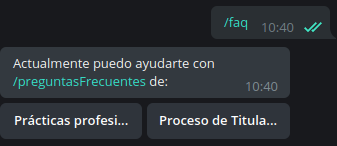
\includegraphics[scale=0.5]{media/imagenes/sc/faq.png}
        \caption[Bot FAQ]{Captura de pantalla del Bot Respondiendo el nuevo comando faq}
        \label{fig:faq}
    \end{figure}

    \par Complementando los flujos de botones se añadieron versiones de comando de las mismas acciones (ver figura \ref{fig:faq}). Además se pueden agregar otras palabras. Pero ambas se procesan de forma completamente diferente (ver sección \ref{imp:refactoring})

    \begin{figure}[h!]
        \centering
        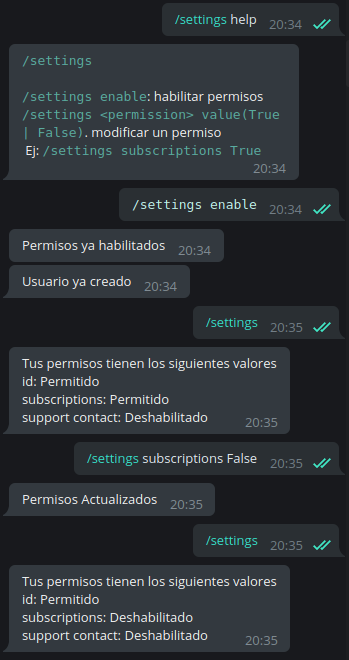
\includegraphics[scale=0.5]{media/imagenes/sc/settings.png}
        \caption[Bot settings]{Captura de pantalla del Bot Respondiendo el nuevo comando settings}
        \label{fig:bot-settings}
    \end{figure}

    \par Además las configuraciones de seguridad y preferencias permiten a los usuarios estar al control de las \textit{features} que requieran, y pueden ser activadas o desactivadas en cualquier momento (ver figura \ref{fig:bot-settings})
    \par Este tipo de configuraciones y funcionalidades, permiten al alumno escoger de que ser informado, segmentar y priorizar la información, y así, se añade valor a este sistema de información.

    \begin{figure}[h!]
        \centering
        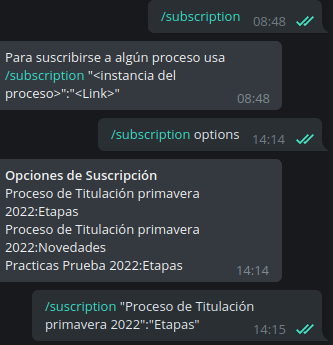
\includegraphics[scale=0.5]{media/imagenes/sc/subscription.png}
        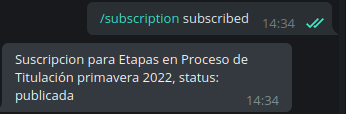
\includegraphics[scale=0.5]{media/imagenes/sc/suscription1.png}
        \caption[Bot subscription]{Captura de pantalla del Bot Respondiendo el nuevo comando subscription}
        \label{fig:bot-sus}
    \end{figure}
    
    \par Se añadió el módulo \textit{BotUsers} a la API, permitiendo que cada alumno pueda escoger la información que es relevante para él. Además ahora puede ser notificado por ejemplo de los plazos de cada proceso. Este módulo contempla que se puedan añadir otras funciones de subscripción como las sugerencias en el futuro. Esto permitiría seguir añadiendo un valor personalizado para cada alumno (ver figura \ref{fig:bot-sus}).

    


\section{Resumen}
    \par De lo expuesto en este capítulo, se puede ver que se satisfacen los requisitos analizado así los cambios necesarios para extender y modificar el sistema, se agregó documentación técnica y lógica al proyecto, se rediseñaron las funcionalidades existentes, y se agregaron nuevas funcionalidades que permiten hacer un sistema extensible, personalizado y confiable.
    \par Además, durante el transcurso del proyecto se sostuvieron conversaciones con las directivas del \acrlong{cadcc}. Y se les presentaron los cambios en el bot, así cómo los problemas de compatibilidad entre otras cosas. El centro de alumnos en conjunto con el memorista anterior, fueron validando los cambios en el código, las nuevas funcionalidades logradas y también apoyaron en la resolución de algunos errores específicos.
    \par Además, cómo se explicita en la memoria, el diseño de las funcionalidades se hizo tomando de forma explícita los objetivos de los alumnos y las cualidades que valoran en estos objetivos.